\section{Sprawdzenie poprawności wartości Upp, Ypp}

Przeprowadzono symulację odpowiedzi procesu dla punktu pracy. 
Ustalone zostało stałe sterowania o wartości Upp = \num{0,8}.
Wynik: 
Uzyskane wyjście procesu jest stałe i wynosi Ypp=\num{2.0}.

\begin{figure}[H]
    \centering
    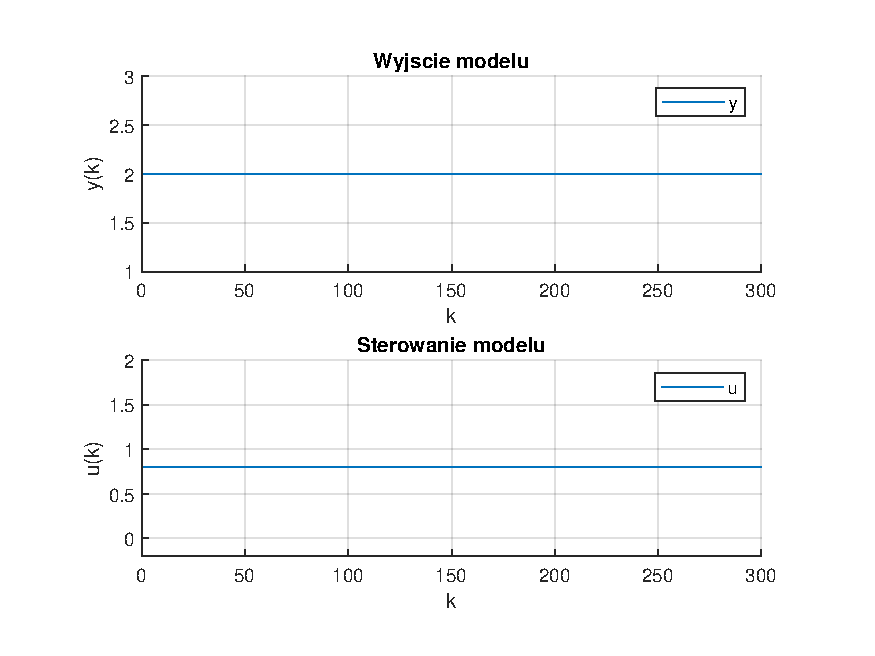
\includegraphics[scale=0.8]{../projekt/zad1/y.pdf}
    \caption{projekt/zad1/y.pdf}
\end{figure}

Wniosek: 
Stała wartość wyjścia oznacza poprawność wartości Upp i Ypp.

